%%%%%%%%%%%%%%%%%%%%%%%%%%%%%%%%%%%%%%%%%%%%%%%%%%%%%%%%%%%%%%%%%%%%%%%%%%%%%%%%%%%%%%%%%%%%%%%%%%%%%%
%
%   Filename    : chapter_2.tex 
%
%   Description : This file will contain your Review of Related Literature.
%                 
%%%%%%%%%%%%%%%%%%%%%%%%%%%%%%%%%%%%%%%%%%%%%%%%%%%%%%%%%%%%%%%%%%%%%%%%%%%%%%%%%%%%%%%%%%%%%%%%%%%%%%

\chapter{Review of Related Literature}
This chapter discusses the features, capabilities, and limitations of existing research, algorithms, or software 
that are related/similar to the thesis.

%  The reviewed works and software must be arranged either in chronological order, or by area (from general to specific).  
% Observe a consistent format when presenting each of the reviewed works. This must be selected in consultation with the prospective adviser.

% \textcolor{red}{DO NOT FORGET to cite your references.}


\begin{comment}
%
% IPR acknowledgement: the contents withis this comment are from Ethel Ong's slides on RRL.
%
Guide on Writing your RRL chapter
 
1. Identify the keywords with respect to your research
      One keyword = One document section
                Examples: 2.1 Story Generation Systems
			 2.2 Knowledge Representation

2.  Find references using these keywords

3.  For each of the references that you find,
        Check: Is it relevant to your research?
        Use their references to find more relevant works.

4. Identify a set of criteria for comparison.
       It will serve as a guide to help you focus on what to look for

5. Write a summary focusing on -
       What: A short description of the work
       How: A summary of the approach it utilized
       Findings: If applicable, provide the results
        Why: Relevance to your work

6. At the end of each section,  show a Table of Comparison of the related works 
   and your proposed project/system

\end{comment}

\section{CAI and Human Factors of Children in Learning Music}

This section explains or show the human factors that are involved when teaching children. This will help us add features, and minimize the mistakes when designing and developing our application, FireflyX.

Technology has been evolving throughout these past years making it more accessible to people \cite{czaja2007impact}. More and more schools have been adapting to the evolution of technology using them as tools for teaching \cite{aqda2011comparative}. As such, CAI applications have been used in classroom settings for students in order to help them visualize objects and understand complex ideas at their own pace \cite{arnold1997computer}. 

CAI applications include guided drills, practice exercises, tutorials, simulations, computer visualization of complex objects, and computer-facilitated communication between students and teachers \cite{arnold1997computer, christmann2000comparative}. These kind of applications increase a student's access to information. They can also be adjusted to the preferences of the student. Many students benefit from the immediate responsiveness of
computer interactions and appreciate the self-paced and private
learning environment \cite{arnold1997computer}.

With the evolution of technology, CAI applications are now available on mobile platforms such as tablets and smartphones. iPads and other forms of tablets are becoming a more common tool for teaching in schools these days \cite{papadakis2017mobile}. An example of a mobile application where FireflyX can get some inspiration from is called SAMI which was developed by \citeA{paule2017music}. The visual cues they used for one of their modes, were for memory development. An example of the game's interface is shown in Figure \ref{fig:sami_memory}. This can be applied to Firefly by designing visual cues that help children visualize music properties. Some examples of these visual cues that can be used in Firefly are how fast the tempo is by the flap of the firefly's wings up and how the size of the body of the firefly can increase or decrease the volume. Since the visual cues play an important role in impacting the learning of the children, however previous studies mentioned that focusing too much on these visual cues for music related CAI applications can ruin sense of rhythm  \cite{pennycook1985computer, chung2017designing}. Using well designed applications can attract the attention of children \cite{chung2017designing} and can also increase the pace of learning \cite{cohen2011young}. We can use this for Firefly by designing the interface and using icons that are attractive to children. Figure \ref{fig:iBuAT_ui} and \ref{fig:ICON_DES} show examples of interfaces that children are more attracted to.



\begin{figure}[H]
    \centering
    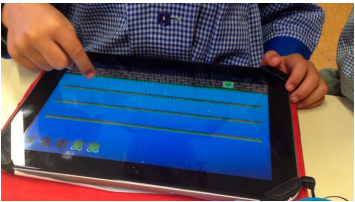
\includegraphics[width=8cm]{figures/sami_interacting.PNG}
    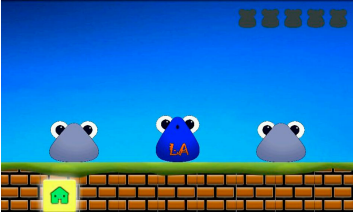
\includegraphics[width=8cm]{figures/sami_memory.PNG}
    \caption{SAMI Application \protect\cite{paule2017music}}
    \label{fig:sami_memory}
    \
\end{figure}

% Having simple layouts can also help ease the use of the application especially for children. According to a feedback for the design of a tool called iBUAT (Paper Prototyping of Interactive Game Design
% Authoring Tool for Children) by \citeA{ibharim2014ibuat}, the children were more attracted to the simple interface that was easy to navigate and understand. Using well designed applications can attract the attention of children \cite{chung2017designing} and can also increase the pace of learning \cite{cohen2011young}. We can use this for Firefly by designing the interface and using icons that are attractive to children. Figure \ref{fig:iBuAT_ui} and \ref{fig:ICON_DES} show examples of interfaces that children are more attracted to.

\begin{figure}[H]
    \centering
    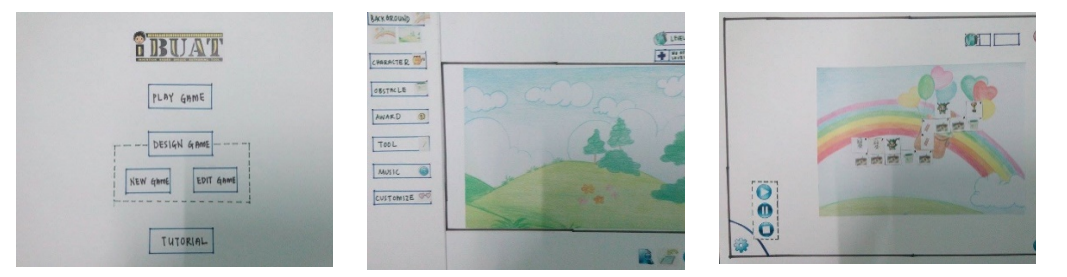
\includegraphics[width=14cm]{figures/iBUAT_design.PNG}
    \caption{iBUAT Interface design \protect\cite{ibharim2014ibuat}}
    \label{fig:iBuAT_ui}
\end{figure}


\begin{figure}[H]
    \centering
    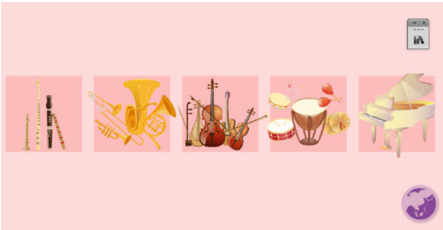
\includegraphics{figures/chung_icons.PNG}
    \caption{Icon Design \protect\cite{chung2017designing}}
    \label{fig:ICON_DES}
\end{figure}

CAI applications have many uses inside and outside school settings, but there are limitations to using it. The results of its effectiveness and quality highly depends on the teaching material and instructional approach \cite{aqda2011comparative}. Making CAI applications must also consider using the student model, which is the acknowledgement of the presence and the limits of the knowledge of the user \cite{self1974student}. This means making multiple levels for difficulties of the CAI application for the user. The sandbox environment or sandbox approach is also another educational tool that lets the users explore the tool and learn how to use it on their own without any instructional procedures like CAI. This allows the application for the users to learn and explore FireflyX for themselves.

%martX
In order for CAI applications to be even developed in the first place, the concept of human factors must be understood. Human factors are defined as a discipline concerned with understanding the interactions among humans and elements of a system in order to be able optimize human well-being when interacting with these systems \cite{salvendy2012handbook}. Experts in the field contribute to the different tasks associated with these systems in order to make these systems have the ability to be compatible with the needs, abilities and limitations of people. 

However, systems not optimized or worse for human interaction are also found to be detrimental to the people using it \cite{foley1984human}. For example a badly designed user interface may lead to negative outcomes. Negative outcomes include lower productivity, increased frustration and the need for redesigning to eliminate these outcomes. Due to this, the need for understanding Human factors arises.

To help maximize the usability of an application, specific human factors related to the application's purpose must be observed. For example, if an application's purpose is to educate, then the factors that should be taken into account are the student's experiences and limitations such as reading capabilities \cite{radu2014augmented}. By knowing the users capabilities, an application can be better used by the users due to it being designed to the users needs or specifications. One specific application of this is scaffolding. Scaffolding is defined as something or someone that provides assistance when a child is acquiring a new skill during the execution of the actual skill itself \cite{strommen1998interface}. However, scaffolding can come in many different forms but finding the most optimal form of scaffolding can be done by understanding the specific user needs and limitations.

Since FireflyX would be assisting in learning music for children, factors in education and children can should be taken into account. A study mentions that these factors include the children's imagination, their media generation and age differences \cite{oosterholt1996interaction}. The importance of imagination comes in involving the children in the concept phase when discussing new products to them. Their generation is important as they wont respond much to things that have nothing to do with their generation. Also their generation usually also makes them have certain skills for using technology compared with other generations. Finally the age differences are important because a child grows fast mentally and physically making them have different views to each other if they are even a few years in age apart.


% \usepackage{color}

% \begin{landscape}
% \begin{table}[]
% \begin{tabular}{|l|l|l|l|}
% \hline
% Authors                                                                                                                                                      & Focus                                                                        & Theory/Principle                                                                      & Contributions/Details                                                                                                                                                                                                                                                                                                                                                                                                         \\ \hline
% \begin{tabular}[c]{@{}l@{}}Aqda, Hamidi, \& Rahimi(2011);\\ Chung, Wu, (2017; Arnold (1997);\\ Barrow, Markman, Rouse (2008);\\ Pennycook(1985)\end{tabular} & \begin{tabular}[c]{@{}l@{}}Computer-aided\\ Instruction\end{tabular}         & \begin{tabular}[c]{@{}l@{}}Advantages and\\ disadvantages\\ of using CAI\end{tabular} & \begin{tabular}[c]{@{}l@{}}CAI gives student a private\\ learning space, assists in \\ teaching in the learning\\ process of children. But \\ Poorly design systems can \\ have big negative effects.\end{tabular}                                                                                                                                                                                                            \\ \hline
% \begin{tabular}[c]{@{}l@{}}Levinowitz (1999);\\ Chung, Wu(2017)\end{tabular}                                                                                 & \begin{tabular}[c]{@{}l@{}}Children Learning\\ using Technology\end{tabular} & Visualization Cues                                                                    & \begin{tabular}[c]{@{}l@{}}We can use visual cues in\\ order to represent music\\ properties for Firefly.\end{tabular}                                                                                                                                                                                                                                                                                                        \\ \hline
% \begin{tabular}[c]{@{}l@{}}Cohen, Hadley, Frank (2011);\\ Chung, Wu (2017)\end{tabular}                                                                      & \begin{tabular}[c]{@{}l@{}}Computer-aided\\ applications\end{tabular}        & Interface Design                                                                      & \begin{tabular}[c]{@{}l@{}}Good interface design and\\ icons can encourage and\\ attract the attention of children\\ to use our application.\end{tabular}                                                                                                                                                                                                                                                                     \\ \hline
% \begin{tabular}[c]{@{}l@{}}Czaja, \& Lee,(2007);\\ qda, Hamidi, \& Rahimi(2011);\\ Self (1974);\\ Aqda, Hamidi, \& Rahimi (2011)\end{tabular}                & \begin{tabular}[c]{@{}l@{}}Computer-aided\\ Instruction\end{tabular}         & \begin{tabular}[c]{@{}l@{}}Importance of\\ Designing CAI\end{tabular}                 & \begin{tabular}[c]{@{}l@{}}The evolution of technology\\ has allowed it to be more accessible\\ and mobile to people. The teaching \\ material and instructional approach \\ greatly affect the quality of education \\ of using computer-aided instruction\\ applications. CAI applications must \\ acknowledge a ”student model”. \\ Difficulty of the instructions depend \\ on the knowledge of the student.\end{tabular} \\ \hline

% \end{tabular}
% \end{table}
% \end{landscape}

% \begin{landscape}
% \begin{table}[]
% \begin{tabular}{|l|l|l|l|}
% \hline
% Authors                                                                       & Focus         & Theory/Principle                                                         & Contributions/Details                                                                                                                                                                                                                                                                                                                                \\ \hline
% Salvendy (2012)                                                               & Human Factors & \begin{tabular}[c]{@{}l@{}}Definition of \\ Human Factors\end{tabular}   & \begin{tabular}[c]{@{}l@{}}Human factors is a discipline that\\ deals with understanding human\\ interaction in order to maximize\\ human well being when designing\\ systems.\end{tabular}                                                                                                                                                          \\ \hline
% Foley, Wallace \& Chan (1984)                                                 & Human Factors & \begin{tabular}[c]{@{}l@{}}Importance of\\ Human Factors\end{tabular}    & \begin{tabular}[c]{@{}l@{}}Systems that do not think about\\ these factors may lead to negative\\ outcomes such as lower productivity\end{tabular}                                                                                                                                                                                                   \\ \hline
% Radu (2014); Stronmen (1998)                                                  & Human Factors & \begin{tabular}[c]{@{}l@{}}Example of Using\\ Human Factors\end{tabular} & \begin{tabular}[c]{@{}l@{}}By researching and understanding \\ the user needs or capabilities, the \\ system can be better used by the\\ users. One application of this is \\ scaffolding. There are many ways to\\ implement scaffolding but  knowing \\ human factors can lead to the best\\ implementation catered to a user\\ need.\end{tabular} \\ \hline
% \begin{tabular}[c]{@{}l@{}}Oosterholt, Kusano \& Vries \\ (1996)\end{tabular} & Human Factors & \begin{tabular}[c]{@{}l@{}}Human Factors of\\ Children\end{tabular}      & \begin{tabular}[c]{@{}l@{}}Children have human factors related \\ to education. These factors include \\ the children's imagination, their \\ media generation and age differences.\end{tabular}                                                                                                                                                     \\ \hline
% \end{tabular}
% \end{table}
% \end{landscape}
\begin{landscape}
\begin{table}[]
\caption{Related Studies on CAI and Human Factors of Children in Learning Music}
\begin{tabular}{|l|l|l|l|}
\hline
Authors                                                                                                                                                                                                                              & Focus                                                                        & Theory/Principle                                                                      & Contributions/Details                                                                                                                                                                                                                                                                                                                                                                                                         \\ \hline
\begin{tabular}[c]{@{}l@{}}Aqda, Hamidi, \& Rahimi(2011);\\ Chung, Wu, (2017; Arnold (1997);\\ Barrow, Markman, Rouse (2008);\\ Pennycook(1985); Cohen, Hadley, \\ \& Frank (2011); Self (1974);\\ Czaja, \& Lee,(2007)\end{tabular} & \begin{tabular}[c]{@{}l@{}}Computer-aided\\ Instruction\end{tabular}         & \begin{tabular}[c]{@{}l@{}}Advantages and\\ disadvantages\\ of using CAI\end{tabular} & \begin{tabular}[c]{@{}l@{}}CAI gives student a private\\ learning space, assists in\\ teaching in the learning\\ process of children. Good designed \\ systems make it more usable for \\ children. Poorly designed systems can \\ have big negative effects. Difficulty \\ of the instructions depend on \\ the knowledge of the student.\end{tabular}                                                                       \\ \hline
\begin{tabular}[c]{@{}l@{}}Levinowitz (1999);\\ Chung, Wu(2017)\end{tabular}                                                                                                                                                         & \begin{tabular}[c]{@{}l@{}}Children Learning\\ using Technology\end{tabular} & Visualization Cues                                                                    & \begin{tabular}[c]{@{}l@{}}We can use visual cues in\\ order to represent music\\ properties for Firefly.\end{tabular}                                                                                                                                                                                                                                                                                                        \\ \hline
\begin{tabular}[c]{@{}l@{}}Salvendy (2012)\\ Foley, Wallace \& Chan (1984)\\ Radu (2014); \\ Stronmen (1998)\end{tabular}                                                                                                            & Human Factors                                                                & \begin{tabular}[c]{@{}l@{}}Definition of\\ Human Factors\end{tabular}                 & \begin{tabular}[c]{@{}l@{}}Human factors is a discipline that\\ deals with understanding human\\ interaction in order to maximize\\ human well being when designing\\ systems. Systems that do not think about\\  these factors may lead to negative\\ outcomes such as lower productivity.\\ By researching and understanding\\ the user needs or capabilities, the\\ system can be better used by the\\ users.\end{tabular} \\ \hline
\begin{tabular}[c]{@{}l@{}}Oosterholt, Kusano \\ \& Vries (1996)\end{tabular}                                                                                                                                                        & Human Factors                                                                & \begin{tabular}[c]{@{}l@{}}Human Factors of\\ Children\end{tabular}     & \begin{tabular}[c]{@{}l@{}}Children have human factors related to \\ education. These factors include\\ the children's imagination, their \\ media generation and age differences\end{tabular}                                                                                                                                                                                                                                \\ \hline
\end{tabular}
\end{table}
\end{landscape}

\section{Sandbox Environment and other Dynamic Interfaces}

This section provides an analysis on how different studies made use of sandbox environments. This will also highlight the results of testing these sandbox environments. It is important that we understand how to properly implement a suitable environment for the children and how to properly conduct testing on them while learning respect to these sandbox environments.

A sandbox environment is an environment, usually set to encourage playfulness, where users can use it as they like. A sandbox environment can be created by implementing the sandbox approach to a software where it is executed it in a specific operating system environment \cite{prevelakis2001sandboxing}. The sandbox approach also encourages users to play boundlessly, thereby increasing their curiosity and engagement in using the environment \cite{goldberg1996secure}.

In the outside world context, children prefer playing games because it stimulates their minds and helps them think creatively \cite{martin1999social, inal2007flow}. The same is also considered in a virtual environment such as an app, children are able to emulate playing outside by using a sandbox environment in an app. The use of apps have been found to increase visual stimulation, improve their navigation skills and be familiarized with music \cite{burton2016music}.

One example of an application that implemented a sandbox approach is Scratch. It allows users to drag and drop blocks to control 2D graphical objects moving on the background, Figure \ref{fig:Scratch_User_Interface} shows a sample of the interface of Scratch. One of the most important feature of Scratch is that it is always live, meaning it requires no compilation step or run mode. Users can also add blocks while a script is running. This lets users be engaged with their projects and always be able to tinker with the blocks \cite{maloney2010scratch}. In the study of \citeA{ouahbi2015learning}, high school students were able grasp programming concepts, and syntax was also not an issue for them. In addition to this, Scratch allows easy visualization of how the algorithm is looks like, and in effect increasing a user’s motivation to learn programming \cite{erol2017effects}. By implementing these features, Scratch is able to provide users a sandbox environment that enables them to learn programming. 

\newpage

\begin{figure}[H]
    \centering
    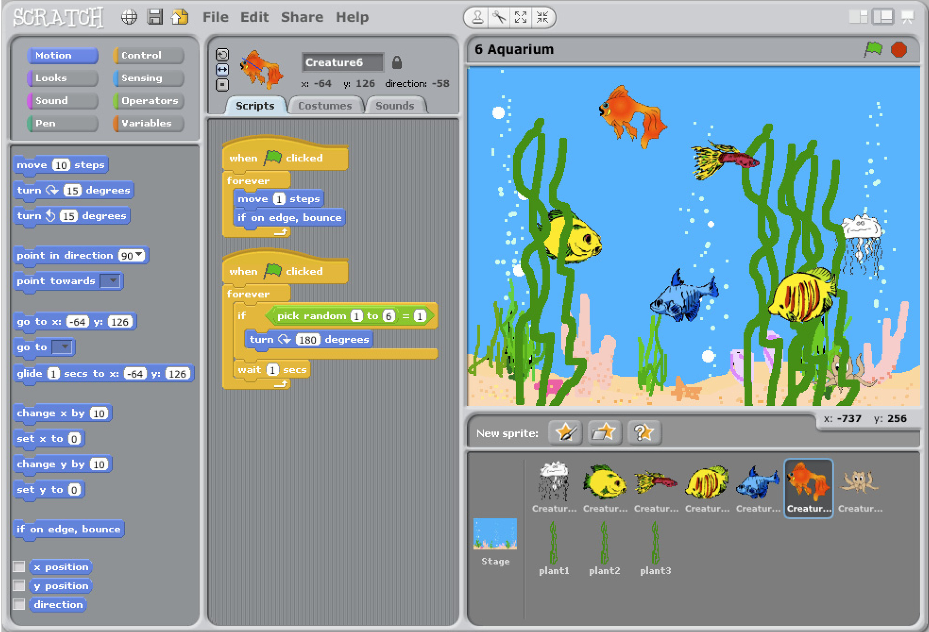
\includegraphics[width=12cm]{figures/Scratch_UI.png}
    \caption{The Scratch User Interface \protect\cite{maloney2010scratch}}
    \label{fig:Scratch_User_Interface}
\end{figure}

Sonification Sandbox was developed in the study of \citeA{walker2003sonification}. It was continued by \citeA{davison2007sonification} and improved on several features and added some new ones as well. It is a graphical toolkit that allows users to map several data sets to timbre, pitch, volume, and pan, with full control over the default, minimum, maximum, and polarity for each attribute. Figure \ref{fig:Sonification_Mappings_Panel} shows a sample interface of the mapping panel and Figure \ref{fig:Sonification_Graph_Panel} shows how the data are graphed. It emulates the sandboxes in playgrounds by making it compatible to all, creating a sandbox that fits all. 

\begin{figure}[H]
    \centering
    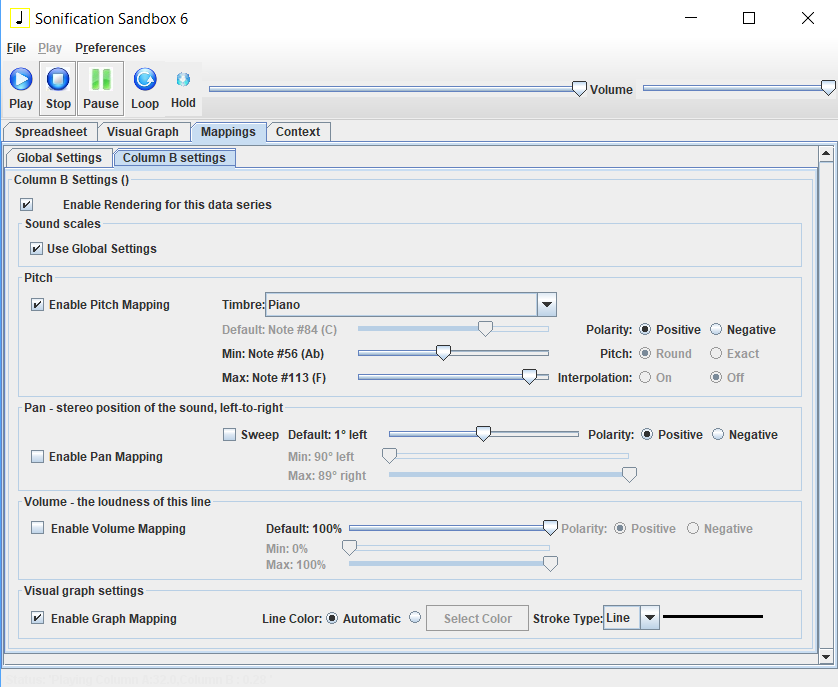
\includegraphics[width=10cm]{figures/Sonification_Mappings_Panel.png}
    \caption{The Mappings Panel for the Sonification Sandbox \protect\cite{walker2003sonification}}
    \label{fig:Sonification_Mappings_Panel}
\end{figure}

\begin{figure}[H]
    \centering
    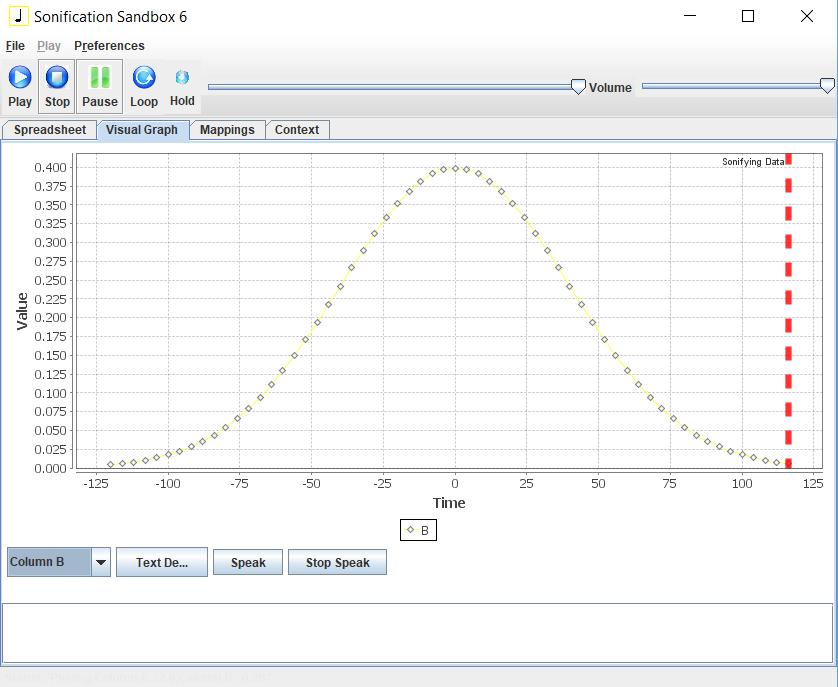
\includegraphics[width=10cm]{figures/Sonification_Graph_Panel.jpg}
    \caption{The Visual Graph Panel for the Sonification Sandbox \protect\cite{walker2003sonification}}
    \label{fig:Sonification_Graph_Panel}
\end{figure}

\newpage

The study of \citeA{paule2017music} developed and evaluated SAMI (Software for music learning in early childhood education). SAMI is a mobile app designed to aid children learning music. The study evaluated SAMI by separating the children into two groups. The control group used Montessori bells, while the experimental group used SAMI. The experimental group was divided into groups of five  and invited to use a tablet in a quiet room outside the classroom with child-sized tables and chairs. The children used SAMI over five sessions divided weekly. Data collection was carried out in four phases. The experiment allotted one session for the children to get familiar with SAMI. The children would have to observe how the mascot moves and sings to each note. The children were then asked questions and when answered correctly the child gets a reward. The second phase observed the children's development of sound discrimination. Phase 3 conducted interviews with the children which was done after three weeks after phase 2. The authors used a semi-structured format asking them which was their favourite game, the one they liked the least and their perception of learning as seen in Figure \ref{fig:children_questionnaire}. In the end, surveys and interviews with children show evidence on the positive effect of technology on children’s motivation and interest for the SAMI group.
% Figure \ref{fig:sami_game1} shows the sample interface of one of the games.
\begin{figure}[H]
    \centering
    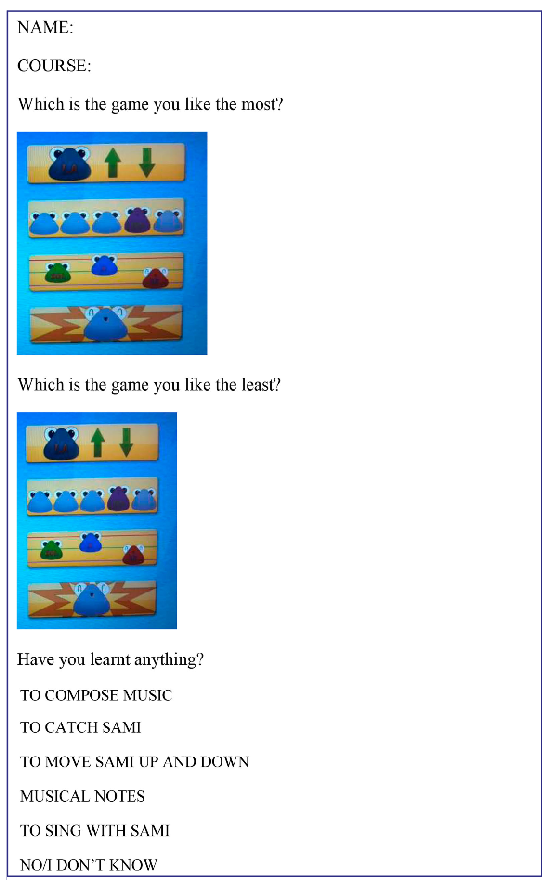
\includegraphics[width=6.5cm]{SAMI_Questionare.png}
    \caption{Children's questionnaire \protect\cite{paule2017music}} 
    \label{fig:children_questionnaire}
\end{figure}
% \begin{figure}[h]
%     \centering
%     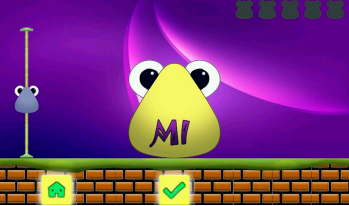
\includegraphics[width=8cm]{sami_game1.PNG}
%     \caption{SAMI Game}
%     \label{fig:sami_game1}
% \end{figure}

\newpage

In the study conducted by \citeA{zhou2011mogclass}, the authors developed and tested MOGCLASS. MOGCLASS is a multimodal collaborative music environment. By using MOGCLASS, teachers are able to manage the classroom better and lets students have a better musical learning environment. In the experiment for MOGCLASS, the music teacher is given a lesson plan which starts with the introduction of the instrument by showing students how to play some notes. Next, the students are asked to answer Q2-Q5 in the questionnaire as seen in table \ref{fig:mogclass_questionnaire}. Afterwards, The student are taught how to play a simple song where the students can make use scaffolding feature. The scaffolding is used to guide people through the usage of devices with the use of visual hints similar to karaoke. After Learning a simple song they are taught an advanced song. Here, the students can still use the scaffolding. The students are then asked to answer Q1 - Q7 of the questionnaire (table \ref{fig:mogclass_questionnaire}). In the final lesson, students are asked to try to perform the advanced song on their own without the use of the scaffolding. After this lesson, the teacher will grade and assess the students in terms of creativity, style and technical proficiency. Lastly, the students are asked to answer the questionnaire once more.

\begin{table}[H]
    \centering
    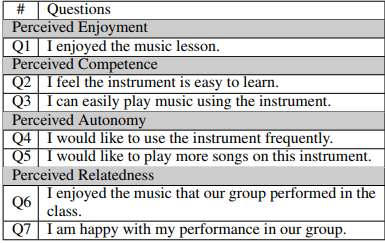
\includegraphics[width=7cm]{mogclass_questionaire.PNG}
    \caption{MOGCLASS Questionnaire \protect\cite{zhou2011mogclass}}
    \label{fig:mogclass_questionnaire}
\end{table}

Xylotism is an interactive game implemented in a sandbox environment that aims to help children learn and teach music to children \cite{elahi2017xylotism}. The study tried to mirror the scenario introduced in the study of \citeA{taheri2016social} where the children trying to learn music is accompanied by a robot and xylophone \cite{taheri2016social}. At the beginning of testing Xylotism, the game's instructions are first described to the child. Then, half of the children were tasked to use the app, while the other half were tasked to use a real xylophone that resembles the app. After 8-12 minutes of playing, the children using the app then switched to using the xylophone, and vice versa. After these, a scenario performed previously by Nima robot \cite{taheri2016social} is simulated, where the instructor plays a rhythm and the child tries his/her best to imitate the instructor. The instructor encourages or warns about the right or wrong answers, respectively. They then used Stambak’s Rhythmic Structures Reproduction test, a test containing 21 easy to hard rhythmic tasks that will assess the participant by having him/her reproduce after hearing \cite{gardner1971children}, in order to gauge how much the child learned.

\label{tab:relBox}
\begin{landscape}
\begin{table}[ht]
\centering
\small
\caption{Related Studies on Sandbox Environments and other Dynamic Interfaces}
\begin{tabular}{|l|l|l|l|} 
\hline
Authors                                                                                                             & Focus                                                                          & Theory/Principle                                                                                                       & Contributions/Details                                                                                                                                                                                                                                                                     \\ 
\hline
\begin{tabular}[c]{@{}l@{}}Prevelakis \& Spinellis (2001);\\Goldberg et al. (1996)\end{tabular}                     & Sandbox Environment                                                            & \begin{tabular}[c]{@{}l@{}}Sandbox environments\\allow users to interact\\with it boundlessly.\end{tabular}            & \begin{tabular}[c]{@{}l@{}}A sandbox approach is \\implemented by executing \\a software in a specific operating\\system environment. This allows\\users to interact with it boundlessly.\end{tabular}                                                                                    \\ 
\hline
\begin{tabular}[c]{@{}l@{}}Marting et al. (1999);\\Inal \& Cagiltay (2007);\\Burton \& Pearsall (2016)\end{tabular} & Children's use of sandboxes                                                    & \begin{tabular}[c]{@{}l@{}}Children prefer playing\\games, in the outside\\world.\end{tabular}                         & \begin{tabular}[c]{@{}l@{}}Children playing games helps them\\think creatively. Being able to play\\without worry stimulates their minds.\\Using apps allow them to emulate this.\end{tabular}                                                                                            \\ 
\hline
\begin{tabular}[c]{@{}l@{}}Walker, Cothran (2003);\\Davidson \& Walker (2007)\end{tabular}                          & \begin{tabular}[c]{@{}l@{}}Sonification in \\sandbox environment \end{tabular} & Sonification                                                                                                           & \begin{tabular}[c]{@{}l@{}}Sonification Sandbox is able to map \\several data sets to timbre, pitch, \\volume, and pan, with full control over\\ each attribute.\end{tabular}                                                         \\ 
\hline
\begin{tabular}[c]{@{}l@{}}Maloney et al. (2010);\\Ouahbi et al. (2015);\\Erol \& Kurt (2017)\\\end{tabular}        & \begin{tabular}[c]{@{}l@{}}Scratch and its sandbox\\environment\end{tabular}   & \begin{tabular}[c]{@{}l@{}}Benefits of Sandbox \\approach\end{tabular}                                                 & \begin{tabular}[c]{@{}l@{}}Scratch is able to help novice learners\\learn programming concepts with\\the use of a sandbox environment.\end{tabular}                                                                                                                                       \\ 
\hline
Paule-Ruiz et al. (2017)                                                                                            & Testing SAMI to children                                                       & \begin{tabular}[c]{@{}l@{}}Children should be\\interviewed and surveyed\\during, and after using the\\app\end{tabular} & \begin{tabular}[c]{@{}l@{}}In-depth process on testing a mobile\\app to children.\end{tabular}                                                                                                                                                                                            \\ 
\hline
Zhou et al. (2011)                                                                                                  & \begin{tabular}[c]{@{}l@{}}Testing MOGCLASS to \\children\end{tabular}         & \begin{tabular}[c]{@{}l@{}}Asking children to answer\\questionnaire should be\\step-by-step\end{tabular}               & \begin{tabular}[c]{@{}l@{}}Children are first shown how to play\\some notes. They are then asked\\some of the questions from the questionnaire.\\After being able to perform simple songs,\\they are again asked some questions. The \\children are then asked to\\answer all the questions.\end{tabular}  \\ 
\hline
\begin{tabular}[c]{@{}l@{}}Elahi et al. (2017);\\Taheri et al. (2016);\end{tabular}                                 & Testing Xylotism to children                                                   & \begin{tabular}[c]{@{}l@{}}Children learn better when\\there is an instructor they\\should follow\end{tabular}         & \begin{tabular}[c]{@{}l@{}}Children are first shown how to use the\\app, after which they are asked to imitate\\the rhythm made by their instructor.\\They are then assessed by using 21\\easy to hard rhythmic tasks.\end{tabular}                                                       \\
\hline
\end{tabular}
\end{table}
\end{landscape}

\section{Review of Related Software}
% This section contains a review of software systems that:
%
% IPR acknowledgement: the following list of items are from Ethel Ong's slides on RRL.
%
% \begin{itemize}
%   \item Belongs to a research area similar to yours
%   \item Addresses a need or domain similar to yours
%   \item Is your predecessor
% \end{itemize}
% \subsection{Perfect Piano}
% Perfect Piano is an application that stimulates a piano and is created by Revontulet Soft Inc. It designed for all ages and can teach how to play the piano by putting labels on piano keys in the screen, then showing corresponding sheet music on top of the screen which shows which keys to press when seeing a specific note. It can also practice a person's skill to listen for melodies and rhythms with a waterfall mode in which keys are seen falling from a height and have to pressed when they reach an appropriate height. 
% %http://www.revontuletsoft.com/
% %https://play.google.com/store/apps/details?id=com.gamestar.perfectpiano

% \subsection{Violin}
% Magical Bow is an application that stimulates a violin and is created by Rubycell. This app teaches users by stimulating a violin and  how to play it, controls include sliding the violin bow up and down to change the note played and sliding the bow side wards to play the note. It helps users learn the proper way to make violin notes by showing them what note they are making when using the bow at a certain angle.
% %https://play.google.com/store/apps/details?id=com.rubycell.violin

% \subsection{Kids Music Instruments Sounds}
% Kids Music Instruments Sounds is an application that multiple simple instruments and is created by Kidstatic Apps.  This app is mainly designed for kids with its simplistic design and simple controls. It shows kids what certain sounds certain instruments play when they are tapped at certain parts. The different instruments for the children to experience include the xylophone, saxophone, drums, and more.
% %http://www.kidstatic.net/
% %https://play.google.com/store/apps/details?id=com.kidstatic.kidsmusicinstruments

% \subsection{iBone}
%  The Pocket Trombone is an application that simulates a trombone and is created by Spoonjack and LLC. It is designed for all ages and teaches the trombone with its multiple Controls that include sliding, wiggling and even blowing into the phone to make music. Learning how to play the trombone is shown by a suggestive program that suggests what notes to be played during a song. If further help is needed, an AI can show the user what the entire song sounds like when the right notes are pressed so they may know if what they are doing is right.
% %http://ibone.spoonjack.com/
% %https://play.google.com/store/apps/details?id=com.spoonjack.ibone&hl=en

There are several music applications that are not sandbox in approach but still provide virtual collaborative environments for expression and composition. One example is the work of \cite{zhou2011mogclass} called MOGCLASS. MOGCLASS is a multimodal collaborative music environment that enhances students’ musical experience and improves teacher’s management of the classroom. This application features an interface for the teacher and a separate interface for the students. The teacher’s interface has features that allow the teacher to manage the class better, while the student’s interface has features that mimic instruments this supports a music technique called scaffolding.

MOGCLASS simulates 3 instruments for the students and can be seen in 3 different student interfaces. The first instrument is called a hitter and it stimulates a drum. It uses an accelerometer in which makes the device detects handshakes and makes a sound proportional to the level of shaking. The second instrument is called a tapper which stimulates a piano. Figure \ref{fig:mogclass_student_interface} also shows how the scaffolding looks like as it is a set of bars that drop down from the top of the screen. The location of the bar shows which note to be played and the size of the bar shows how long the note should be played. The last instrument is the slider and it stimulates a violin. The vertical position of the finger plays different notes on the slider. Figure \ref{fig:mogclass_student_interface} shows the sample student interface of the second instrument which represents the piano.

\begin{figure}[H]
    \centering
    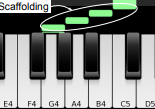
\includegraphics[width=8cm ]{mogclass_studen_interfaces.PNG}
    \caption{MOGCLASS Student Interface \protect\cite{zhou2011mogclass}}
    \label{fig:mogclass_student_interface}
\end{figure}

As for the teacher’s interface which is shown in figure \ref{fig:mogclass_teacher_interface}, it comes with many features that can help manage the class. The teacher can control which instrument the student’s interface will display and which notes it can start with. The teacher can also control if the student is muted or not. Finally, the teacher can choose which song will be used when scaffolding is used in the student’s interface.

\begin{figure}[H]
    \centering
    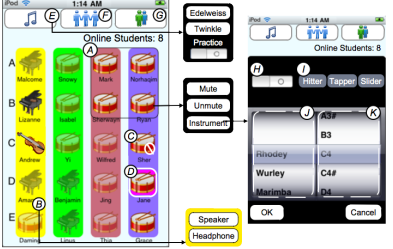
\includegraphics[width=8cm ]{mogclass_teacher_interace.PNG}
    \caption{MOGCLASS Teacher Interface \protect\cite{zhou2011mogclass}}
    \label{fig:mogclass_teacher_interface}
\end{figure}

%The experiment to test out MOGCLASS adopts a between-subjects design which is a experiment where there are multiple groups in which each group is tested in a different way to compare results. The independent variable was the musical instrument. One class was taught with MOGCLASS and the other class was taught with recorders while all other variables were kept constant such as the teacher and the lesson plan. For the duration of the lesson, parts of the questionnaire will be filled up afterwards. 

%The lesson plan of the music teacher starts with introduction of the instrument by teaching how to play the some of the notes (Allow students to answer Questionnaire Q2 - Q5). Afterwards, The student are taught how to play a simple song in which the MOGCLASS students can use scaffolding. Scaffolding is used to guide people through the usage of devices with the use of visual hints similar to karaoke. After Learning a simple song they are taught an advanced song and here the MOGCLASS students can still use the scaffolding (Allow students to answer Questionnaire Q1 – Q7). In the final lesson, students are to try to perform the advanced song on their own and the MOGCLASS students cannot use scaffolding. After this lesson, the teacher will grade and assess the students in terms of creativity, style and technical proficiency and the students will fill up the questionnaire once more (Allow students to answer Questionnaire q1-q1).

%The questionnaire as seen in Figure \ref{fig:mogclass_questionnaire} is divided into 4 parts, enjoyment, competence, autonomy, and relatedness. Each question was rated on a 7- point Likert scale. Results from the experiment and the questionnaires showed that MOGCLASS achieves what is was made for which is effective in motivating students to learn music, improving the way they collaborate with other students as well as helping teachers manage the classroom.

From this application, FireflyX can make use of the scaffolding feature in order to help guide children in learning musical elements. Having a separate teacher and student interface may also be taken into consideration since teachers may help accelerate the learning of the children as well. 

%MOGCLASS
% https://sci-hub.tw/https://dl.acm.org/citation.cfm?id=1979016&fbclid=IwAR03o9hxpQ1LsxIX_NsdQ7fQtPRK31aKool3jAPYeUDz3TIxAz8chPiXrcc

Aside from MOGCLASS, More scaffolding can be found in a study by \citeA{jorgensen2015mobile}. This includes virtual instruments for children so that they may engage more in museum setups. The application has three instruments to use being the harpsichord, double bass and the viola. The application suggests using them one by one and in the end all past performances are played back simultaneously revealing that playing instruments together make a composition. All the instruments have colored rectangles that scroll downwards which depicts the note they should be playing. These rectangles are a form of scaffolding.

For the harpsichord, the colored rectangles are above a keyboard and the rectangles determine which key should be pressed for the correct note to be played. For the double bass, there are colored strings below and the colored rectangles refer to which string has to be plucked in order to play the correct note. The viola, is similar to the double bass but instead of plucking, children have to swipe on the correct string in order to stimulate using a bow and to play the correct note. FireflyX might be able to use the different forms of scaffolding presented here. We can also make use of the way this application simultaneously plays different instruments at once for when there are multiple fireflies created.

%  responses may serve as a way to guide the users if they are doing correct or not. Firefly may be able to use the feedback system given my Nima to motivate children further in their usage of Firefly.\begin{figure}[Theseh]
%     \centering
%     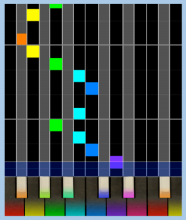
\includegraphics[width=8cm \textwidth]{museum_harpsichord.PNG}
%     \caption{Music Authoring Application \protect\cite{jorgensen2015mobile}}
%     \label{fig:museumHarpsichord}
% \end{figure}

% \begin{figure}[h]
%     \centering
%     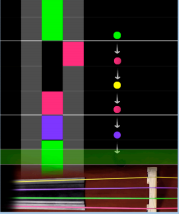
\includegraphics[width=1 \textwidth]{museum_double_bass.PNG}
%     \caption{Music Authoring Application \protect\cite{jorgensen2015mobile}}
%     \label{fig:museumBass}
% \end{figure}

% \begin{figure}[ht]
%     \centering
%     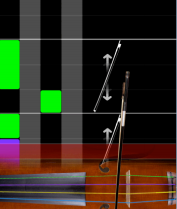
\includegraphics[width=8cm ]{museum_viola.PNG}
%     \caption{Viola Interface \protect\cite{jorgensen2015mobile}}
%     \label{fig:museumViola}
% \end{figure}

% A Mobile Music Museum Experience for Children
% https://nime2015.lsu.edu/proceedings/267/0267-paper.pdf

The development of musical tools have migrated to mobile environments as well. One study is SAMI by \cite{paule2017music}. SAMI is a music learning application for children using tablet-computers. For it to be able to teach music, it has 4 games that are designed to facilitate learning and encourage children's thinking and creativity. SAMI, a triangular blob with large eyes, is also the mascot of the game and is interacted with in all of the games. The first game aims to educate the children by using the ears to identify several sounds. In short, the first game is a memory game using notes. The game plays a note and the task of the user is to tap SAMI with a similar noise representing that note. Each SAMI has a color at first to determine the note. The second game is a memory game with order of the notes wherein the children have to tap on SAMIs in the correct order. This aims to teach notes as if they were part of a major chord. The third game is a reactive tapping game and aims to teach fine motor skills required to play instruments. There are 3 rows and each location of SAMI places a different note. SAMIs appear and the child needs to tap on SAMI before they disappear. SAMIs on the top row play higher pitched notes when tapped. The last game is a composing game which combines all the previous games and has the child try to compose with SAMIs by having arrange SAMI’s in different heights and at a certain arrangement. These games may serve as an inspiration on how some features or parts of FireflyX may be able to be implemented.


% Music learning in preschool with mobile devices (SAMI)
% https://sci-hub.tw/https://doi.org/10.1080/0144929X.2016.1198421


Just as SAMI teaches with its games, an application by \citeA{elahi2017xylotism} also teaches with instructions. This application features a bot named Nima that gives instructions. The instructions given by Nima follow a step by step process. The initial stages would be instructions to get the user to understand notes. These instructions include commands for the user to do something or questions to ask the user. The later stages would involve trying to make the user replicate rhythms. 

Based on the user's actions, Nima also gives some feedback to help guide the user. When the user is doing well, Nima can respond by doing dances and saying things like that's great, bravo, etc. If the user makes a mistake, Nima says things like pay attention or try again. Aside from these responses, there are also emojis showing happy faces or sad faces depending on the user's actions as well. From this application, FireflyX may be able to use the instructions and feedback system given by Nima. The instruction system may help guide the children on the usage of FireflyX. The feedback system may encourage the children with their usage of FireflyX.

%Xylotism
%https://sci-hub.tw/https://link.springer.com/chapter/10.1007/978-3-319-70022-9_72


Aside from Xylotism, there are other musical applications where children’s preferences are considered especially in measuring engagement or fun. One study is by \citeA{burton2016music}. Common application preferences by children include easy to navigate menus, a variety of ways to engage, visual stimulation, familiar musical material, music that continues without manipulation, and animated characters such as animals, babies, children, movement, and/or dancing.

A table in the study as seen in Table \ref{fig:child_checklist} shows different applications wherein the applications in bold are considered the child friendly applications while the italicized ones aren’t. The table also shows if the application has features that children like. The less child friendly apps are similar to the child friendly app above it in regards on what it aims to teach. 


\begin{table}
\centering
\caption{Child Friendly Features Checklist \protect\cite{burton2016music}}
\label{fig:child_checklist}
\scalebox{0.8}{\begin{tabular}{|l|l|l|l|l|l|l|} 
\hline
Application                   & Characters                            & Movement                              & Dancing                               & Animation                             & Children                              & Songs                                  \\ 
\hline
\textbf{Juno's Piano}         &                                       & \textcolor[rgb]{0.133,0.133,0.133}{\checkmark} & \textcolor[rgb]{0.133,0.133,0.133}{\checkmark} & \textcolor[rgb]{0.133,0.133,0.133}{\checkmark} &                                       &                                        \\ 
\hline
\textit{Virtuoso Piano}       &                                       &                                       &                                       &                                       &                                       &                                        \\ 
\hline
\textbf{Monkey Drum}          & \textcolor[rgb]{0.133,0.133,0.133}{\checkmark} & \textcolor[rgb]{0.133,0.133,0.133}{\checkmark} & \textcolor[rgb]{0.133,0.133,0.133}{\checkmark} & \textcolor[rgb]{0.133,0.133,0.133}{\checkmark} &                                       &                                        \\ 
\hline
\textit{Percussive}           &                                       &                                       &                                       &                                       &                                       &                                        \\ 
\hline
\textbf{Toca Band}            & \textcolor[rgb]{0.133,0.133,0.133}{\checkmark} & \textcolor[rgb]{0.133,0.133,0.133}{\checkmark} & \textcolor[rgb]{0.133,0.133,0.133}{\checkmark} & \textcolor[rgb]{0.133,0.133,0.133}{\checkmark} & \textcolor[rgb]{0.133,0.133,0.133}{\checkmark} &                                        \\ 
\hline
\textit{Loopseque}            &                                       &                                       &                                       & \textcolor[rgb]{0.133,0.133,0.133}{\checkmark} &                                       &                                        \\ 
\hline
\textbf{Ambient Mood}         & \textcolor[rgb]{0.133,0.133,0.133}{\checkmark} & \textcolor[rgb]{0.133,0.133,0.133}{\checkmark} &                                       & \textcolor[rgb]{0.133,0.133,0.133}{\checkmark} &                                       &                                        \\ 
\hline
\textit{Bloom HD}             &                                       &                                       &                                       &                                       &                                       &                                        \\ 
\hline
\textbf{Kids Song Collection} & \textcolor[rgb]{0.133,0.133,0.133}{\checkmark} & \textcolor[rgb]{0.133,0.133,0.133}{\checkmark} &                                       & \textcolor[rgb]{0.133,0.133,0.133}{\checkmark} & \textcolor[rgb]{0.133,0.133,0.133}{\checkmark} & \textcolor[rgb]{0.133,0.133,0.133}{\checkmark}  \\ 
\hline
\textit{iTunes Collection}    &                                       &                                       &                                       &                                       & \textcolor[rgb]{0.133,0.133,0.133}{\checkmark} & \textcolor[rgb]{0.133,0.133,0.133}{\checkmark}  \\ 
\hline
\textbf{Lily Rock Band}       & \textcolor[rgb]{0.133,0.133,0.133}{\checkmark} & \textcolor[rgb]{0.133,0.133,0.133}{\checkmark} & \textcolor[rgb]{0.133,0.133,0.133}{\checkmark} & \textcolor[rgb]{0.133,0.133,0.133}{\checkmark} & \textcolor[rgb]{0.133,0.133,0.133}{\checkmark} & \textcolor[rgb]{0.133,0.133,0.133}{\checkmark}  \\ 
\hline
\textit{Rockmate}             &                                       &                                       &                                       &                                       &                                       &                                        \\
\hline
\end{tabular}}

\end{table}

The first two apps for example aim to teach melody according to the study. The first application, Juno’s Piano is treated by the study as the child friendly application due to it having the features normally preferred by children as seen in the table. In Figure \ref{fig:iPad_friendly}, the application has bright colors and a cute character on top of the piano. 

\begin{figure}[H]
    \centering
    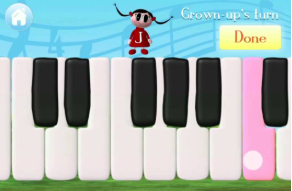
\includegraphics[width=10cm]{ipad_kid_friendy.PNG}
    \caption{iPad Kid Friendly Example \protect\cite{burton2016music}}
    \label{fig:iPad_friendly}
\end{figure}

However, Virtuoso Piano is missing these preferences thus making the study treat it as the less child friendly application. In figure \ref{fig:iPad_unfriendly}, the application is missing characters and only has some dull colors to it. 

\begin{figure}[H]
    \centering
    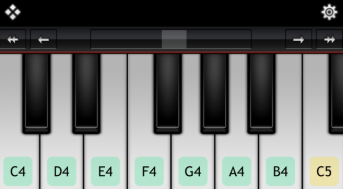
\includegraphics[width=8cm]{ipad_not_kid_friendly.PNG}
    \caption{iPad Not Kid Friendly Example \protect\cite{burton2016music}}
    \label{fig:iPad_unfriendly}
\end{figure}

In order for children to use FireflyX longer, FireflyX will use some features, which will be tested through the different iterations, that children find appealing as seen from the child friendly applications and try to avoid missing some features such as the less child friendly applications.

%ipad prefences
% https://sci-hub.tw/https://doi.org/10.1177/1321103X16642630

Not all applications may be usable for all children however. Some children such as the one’s diagnosed with autism spectrum disorders may be in need of social skills so that they may be able to live independently when they reach adulthood. A study by \citeA{hourcade2012multitouch}, includes the creation of applications in order to promote social skills to these children. One of the applications created was a music authoring application. 

The application has a harp like screen and the children are able to choose tiles which determine what note they would play, the notes on the higher part of the screen depicting higher notes and vice versa. The notes are played in sequence, with the note that is currently played turning green. Since this application aims to promote social skills as well, the music authoring app was designed to be used by multiple children. The multi-touch feature where it can have multiple notes selected at once makes it possible for children to edit at once. 

Since the study also shows that the children mentioned using the application makes it more enjoyable. FireflyX may be able to incorporate the collaborative multi touch feature this application presents as it may attend to more than one children at once so that FireflyX maybe more enjoyable for children.
%This application would be used for collaborative music creation in which children are asked to put a few notes before passing the tablet to another kid. This is for the children to appreciate social interaction. Feedback from the children related to the application is that the music authoring was the best part among the multiple applications and they liked the song they made with their friends. However they also commented that they wanted more instruments. It is found out that technology may be enough of an incentive to improve the quality of social interactions.

% \begin{figure}[!htb]
%     \centering
%     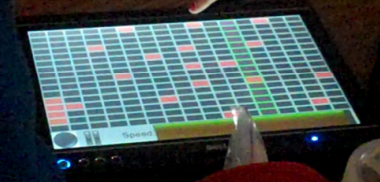
\includegraphics[width=13cm]{music_authoring.PNG}
%     \caption{Music Authoring Application \protect\cite{hourcade2012multitouch}}
%     \label{fig:musicAuthoring}
% \end{figure}


% Multitouch tablet applications and activities to enhance the social
% skills of children with autism spectrum disorders
% https://sci-hub.tw/https://dl.acm.org/citation.cfm?id=2125154


% Mart's Synthesis Table
\begin{landscape}
\begin{table}
\centering
\caption{Related Systems for Children Music Learning Tools}
\begin{tabular}{|l|l|l|l|} 
\hline
Authors                                                                                                                                                                                      & Name of System                                                                         & Platform                                                                            & Comments/Findings                                                                                                                                                                                                     \\ 
\hline
\begin{tabular}[c]{@{}l@{}}Percival et al. (2011);\\ Jorgensen et al. (2015)\end{tabular}                                                                     & \begin{tabular}[c]{@{}l@{}}MOGCLASS;\\ A Mobile Music \\Museum \\Experience \\for Children\end{tabular}           & \begin{tabular}[c]{@{}l@{}}Ipod Touch; \\ Tablet\end{tabular}                         & \begin{tabular}[c]{@{}l@{}}Both show basic scaffolding for various\\ instruments.The first system features \\a separate teacher and student interface. \\The second combines music played and \\plays it back to the user.\end{tabular}                         \\ 
\hline
\begin{tabular}[c]{@{}l@{}} Burton \& Pearsall (2016)\\\end{tabular}                                                      & \begin{tabular}[c]{@{}l@{}}NA \end{tabular}         & \begin{tabular}[c]{@{}l@{}}Ipad \end{tabular}                       & \begin{tabular}[c]{@{}l@{}}It differentiates popular kid-friendly \\applications and less kid-friendly \\applications using common preferences\\ by kids in applications. \end{tabular}  \\ 
\hline
\begin{tabular}[c]{@{}l@{}}{\'A}lvarez-Garc{\'\i}a et al. (2016);\\ Ahmadi et al. (2017) \end{tabular}                                                           & \begin{tabular}[c]{@{}l@{}}SAMI;\\ Xylotism \end{tabular} & Tablet                                                                        & \begin{tabular}[c]{@{}l@{}}Both systems have integrated learning \\music in a step by step process by using \\games. They both use child friendly graphics \\and motivation for the child as they \\learn musical concepts. \end{tabular}                                                                                                   \\ 
\hline
\begin{tabular}[c]{@{}l@{}}Bullock-Rest, Hansen,  \& \\Hourcade(2011)\\ \end{tabular} & \begin{tabular}[c]{@{}l@{}}Music Authoring \\ Application \end{tabular}        & Tablet                                                                           & \begin{tabular}[c]{@{}l@{}}Focusses on an application made for social \\interaction. The application aims for children \\to make music together on a harp like screen. \end{tabular}                                                                        \\ 
% \hline                                                \\
\hline
\end{tabular}
\end{table}
\end{landscape}